\chapter[Metodologia]{Metodologia}
A metodologia adotada neste trabalho se caracteriza pela análise bibliográfica e
pelas características de um estudo de caso para a Medição de TD na proposta de
de \cite{td} uma estratégia de gestão de débito técnico.

\section{Seleção Metodológica}
A pesquisa se caracteriza como descritiva, na qual os pesquisadores analisam o problema
a fim de desenhar um plano de medição codizente com o GQM, tendo como focos
principais o processo e o seu significado,
buscando estabelecer relações entre variáveis e descrevendo características de
um fenômeno.

O intuito foi responder as seguintes questões de pesquisa:

\begin{itemize}
  \item Como traçar um plano de medição para aferir a quantidade de Débito Técnico
  presente?

  \item Como monitorar a qualidade do código, a partir do Débito Técnico, na
  contratação de softwares de terceiros, de forma quantitativa?
\end{itemize}

Como procedimentos de coleta de dados, optou-se pela técnica de estudo de caso
único. Para o diagnóstico da situação, realizou-se a caracterização do órgão por
meio das técnicas de coleta de dados documental, observação participante e
entrevistas semi-estruturadas.

\section{Estudo de Caso}
O objeto de estudo de caso deste trabalho é um órgão público federal brasileiro,
o Ministério das Comunicações (MC). O MC utiliza-se de terceiros para prestação
de alguns serviços quanto às atribuições de TI, entre elas, a contratação de
Fábricas de Softwares (FS) e de apoio a Garantia de Qualidade dos Serviços de TI.

O desenvolvimento de novos projetos por uma FS é executado de acordo com o processo
de gestão de demandas de contratação de desenvolvimento de software por terceiros, s
egundo o SCRUM - GEDDAS (citado em \cite{souza}).

No GEDDAS, após as entregas intermediárias de software, que ocorrem no término de
cada release, realiza-se a macro atividade Atestar Qualidade da Release como pode
ser visto na Figure \ref{fig:geddas}.

\begin{figure}[h]
  \centering
  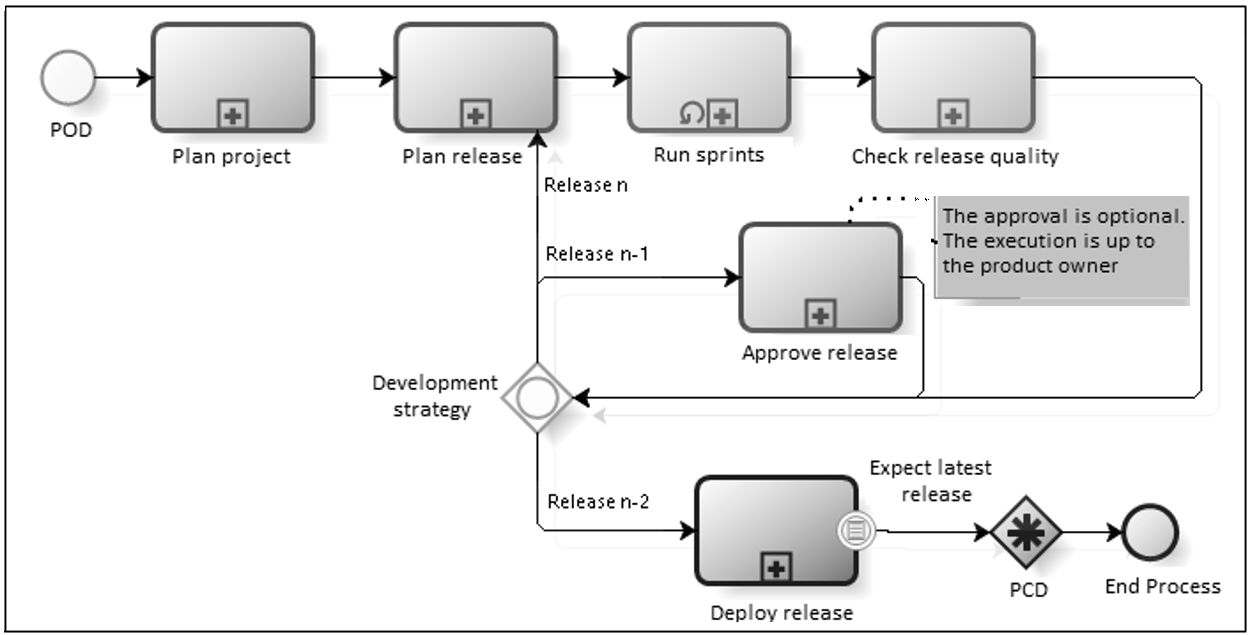
\includegraphics[width=400px, scale=1]{figuras/geddas}
  \caption{GeDDAS Macro Process}
  \label{fig:geddas}
\end{figure}

A atividade Atestar Qualidade da Release possui a atividade Verificar Qualidade
do Incremento de Software,  representada na Figure 2, responsável por verificar a
qualidade do software adquirido pelo terceiro contratado, de acordo com os níveis
mínimos estabelecidos nos critérios de aceite do processo de contratação do
Ministério das Comunicações.

\begin{figure}[h]
  \centering
  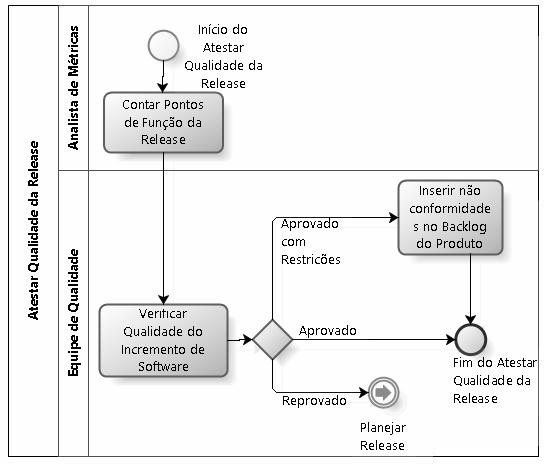
\includegraphics[width=275px, scale=1]{figuras/atestarqualidade}
  \caption{Atestar Qualidade da Release - Sub Processo}
  \label{fig:atestarqualidade}
\end{figure}
